\documentclass[/Users/ikedahajime/GitHub/reserch/master_report/thesis]{subfiles}
% このファイル内だけのコマンド
\begin{document}
\chapter{結果}
\section{はじめに}
本章では計算結果および解析結果を述べる。%TODO:節構成第n節では〜
\section{円に拘束されたABP}
\subsection{系全体のダイナミクス}
m依存、rho依存
\begin{figure}[htbp]
    \centering
    \begin{tabular}{c}
        \begin{minipage}{0.8\hsize}
            \text{(a)}
            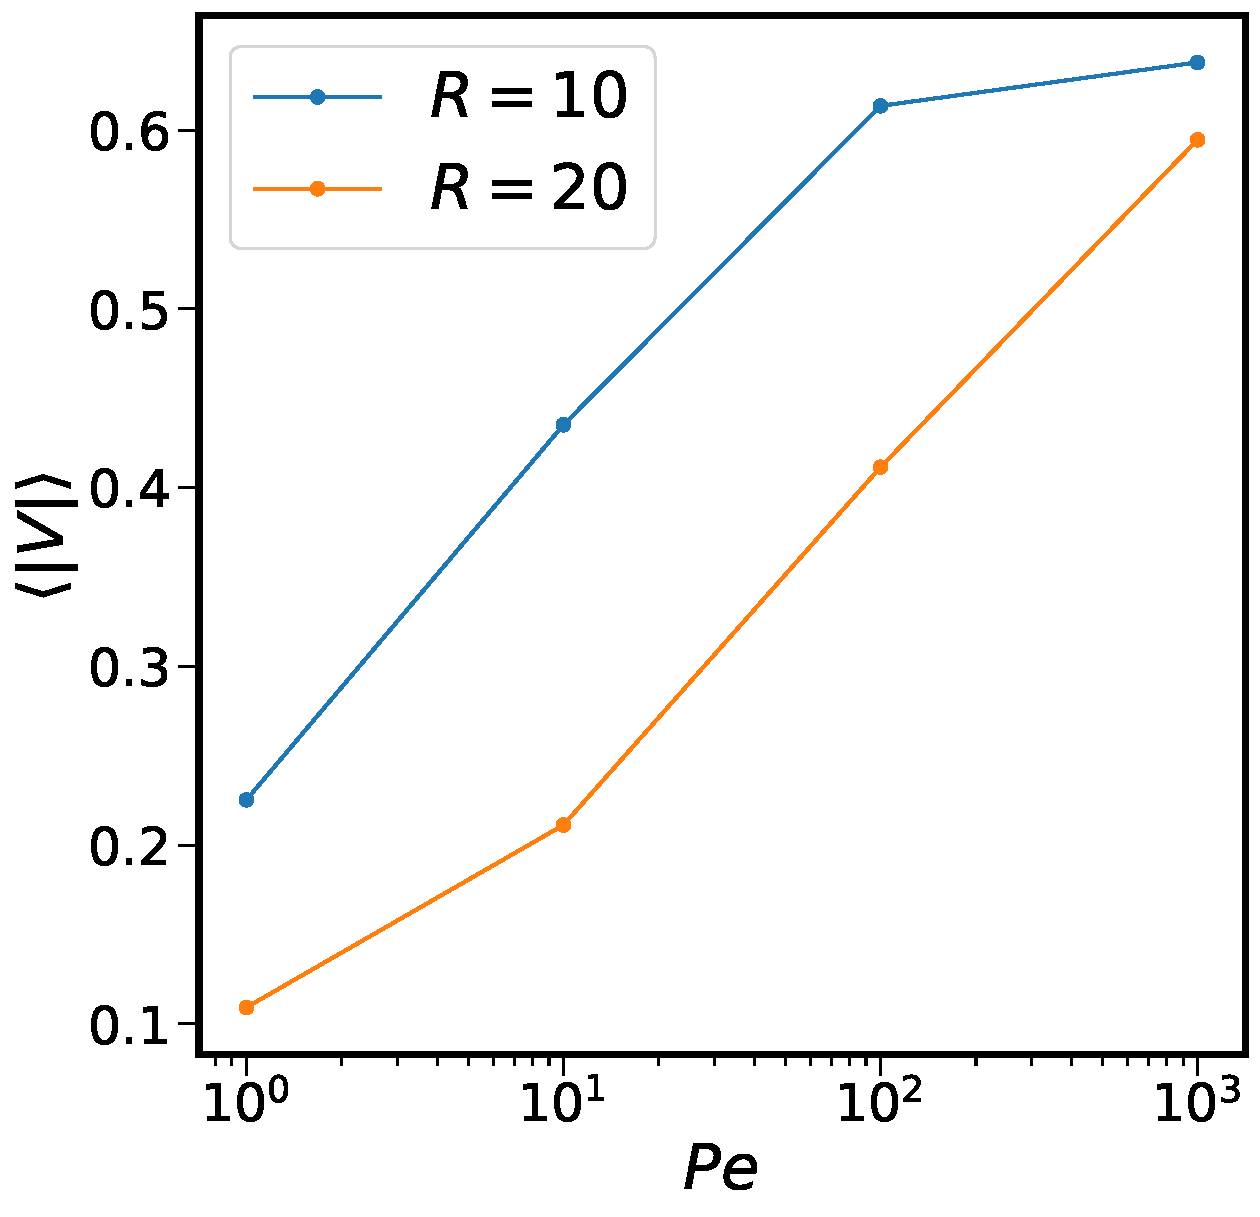
\includegraphics[width=\textwidth]{img/nabp/ens_r1/|V|_0.7_0.1.pdf}
        \end{minipage}
    \end{tabular}
    \caption[Four sample images]
    {
        $|V|$の変化。$\varphi=0.7、M=0.1$
    }
    \label{fig:nabp_vabs_lo0.7}
\end{figure}
\subsection{時間依存性}
生の時間依存
フーリエ変換
\begin{figure}[htbp]
    \centering
    \begin{tabular}{c}
        \begin{minipage}{0.8\hsize}
            \text{(a)}
            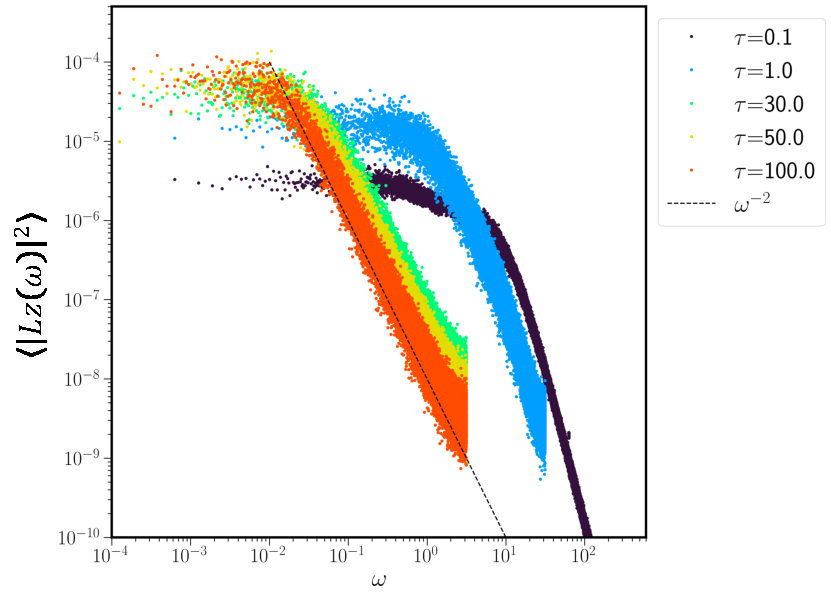
\includegraphics[width=\textwidth]{img/nabp/ens_r1/fig_ft_lz.pdf}
        \end{minipage}
    \end{tabular}
    \caption[Four sample images]
    {
        hoge
    }
    \label{fig:fourie_transform}
\end{figure}
\end{document}
